\chapter{Generazione dei Segnali Principali}

%--------------------------------------------------------------------------------------------

Per la generazione dei segnali a rampa e a triangolo si decide di procedere in ogni caso
per via digitale, utilizzando dei contatori binari abbinati ad un convertitore
digitale-analogico.

%--------------------------------------------------------------------------------------------

\section{Rampa}

%--------------------------------------------------------------------------------------------

\subsection*{Principio di Funzionamento}

%--------------------------------------------------------------------------------------------

Per il segnale a rampa si fa uso di un contatore unidirezionale, ovvero un dispositivo
in grado di contare automaticamente da $0$ a $2^n$ (con $n$ numero di bit) semplicemente
fornendo un segnale di clock adeguatamente dimensionato. Maggiore il numero di bit,
maggiore la precisione del nostro segnale, quindi minore l'intensità del rumore generato.

\begin{figure}[H]
    \centering

    \begin{subfigure}{.5\textwidth}
        \centering
        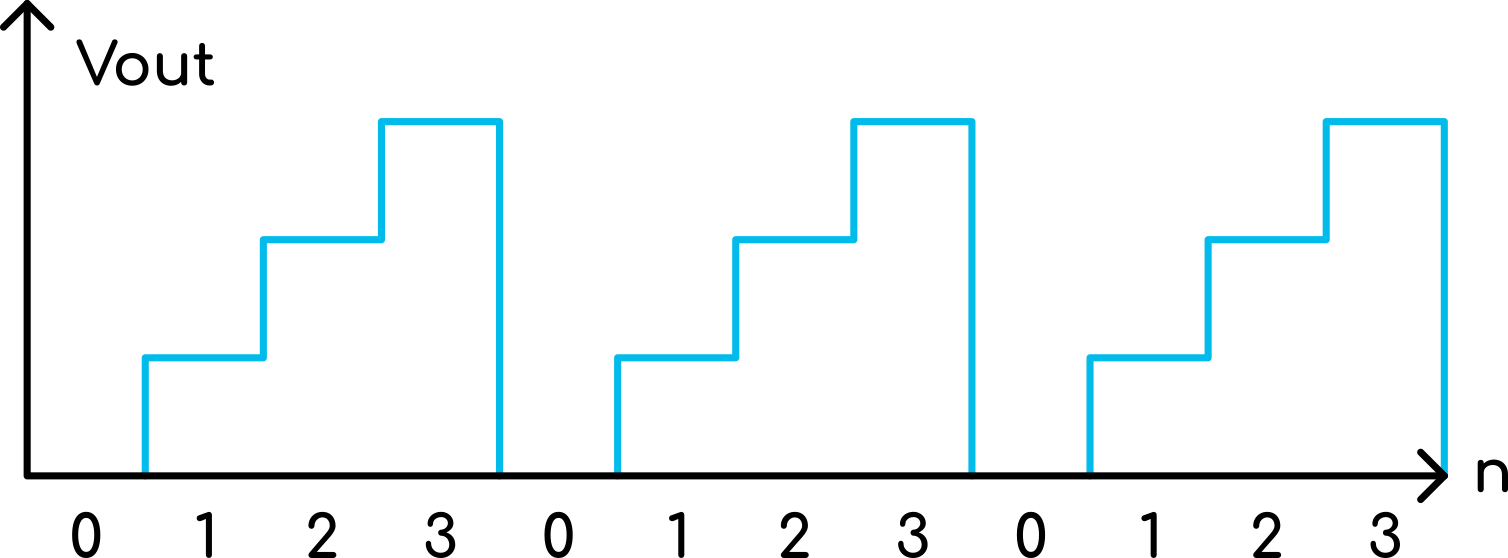
\includegraphics{graphs/low_res_ramp.png}
        \caption{Rampa ottenuta con un contatore a 2 bit}
        \label{low_res_ramp}
    \end{subfigure}%
    \begin{subfigure}{.5\textwidth}
        \centering
        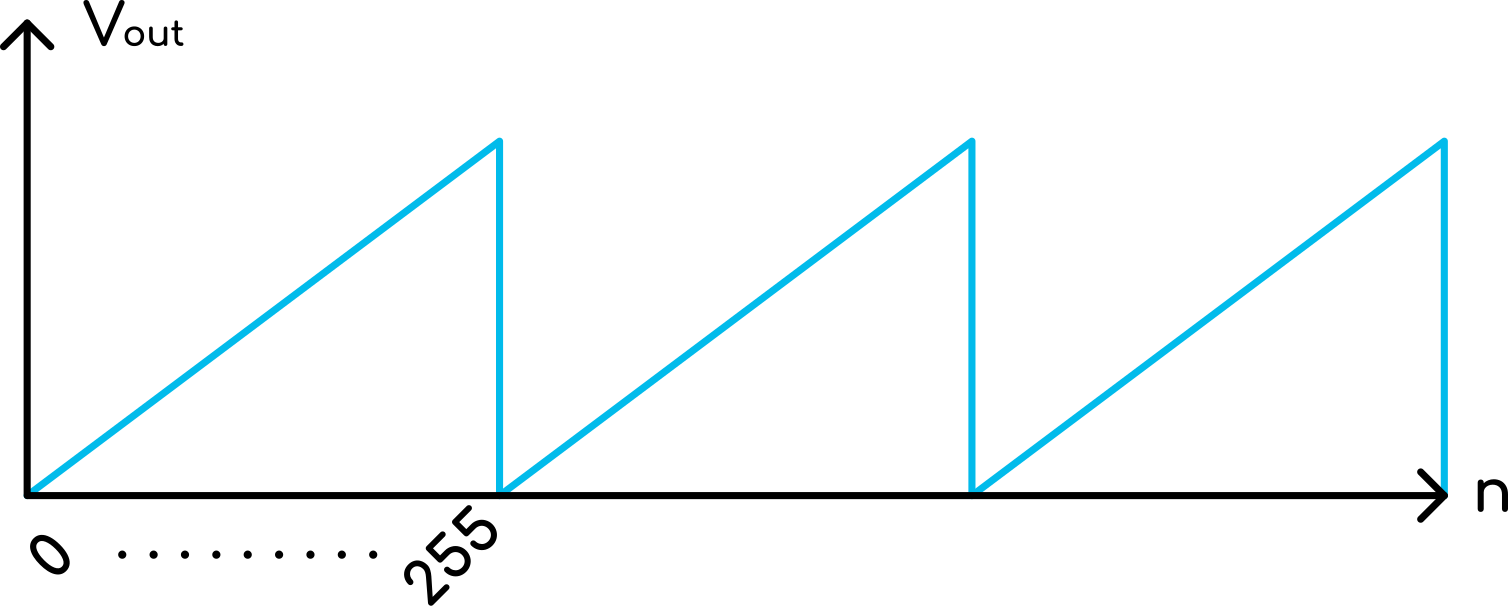
\includegraphics{graphs/high_res_ramp.png}
        \caption{Rampa ottenuta con un contatore a 8 bit}
        \label{high_res_ramp}
    \end{subfigure}

    \caption{Confronto tra contatori unidirezionali con diverso numero di bit}
    \label{ramps}
\end{figure}

Tuttavia aumentando il numero di bit del contatore è facile intuire che, a parità di
frequenza del segnale in uscita, la frequenza del segnale di clock debba necessariamente
aumentare, vale infatti la seguente relazione:

\begin{displaymath}
    f_{signal}=\frac{f_{clk}}{2^n}\ [Hz]
\end{displaymath}

poichè il contatore deve effettuare un conteggio completo durante un periodo del segnale
in uscita. Questo implica dunque un limite massimo al numero di bit del contatore.

La quantità di bit utilizzati per l'applicazione è $8$, valore che ci consente di limitare
al $MHz$ la frequenza di clock, contare fino a $255$ e dividere l'intervallo di tensione
d'uscita in altrettanti livelli, ottenendo quindi una variazione di

\begin{displaymath}
    V_{step}=\frac{2\cdot V_{ref}}{2^n}=\frac{10}{256}\approx39\ mV
\end{displaymath}


per ogni singolo bit (scegliendo $V_{ref}=+5\ V$).
\medskip

\begin{figure}[H]
    \centering
    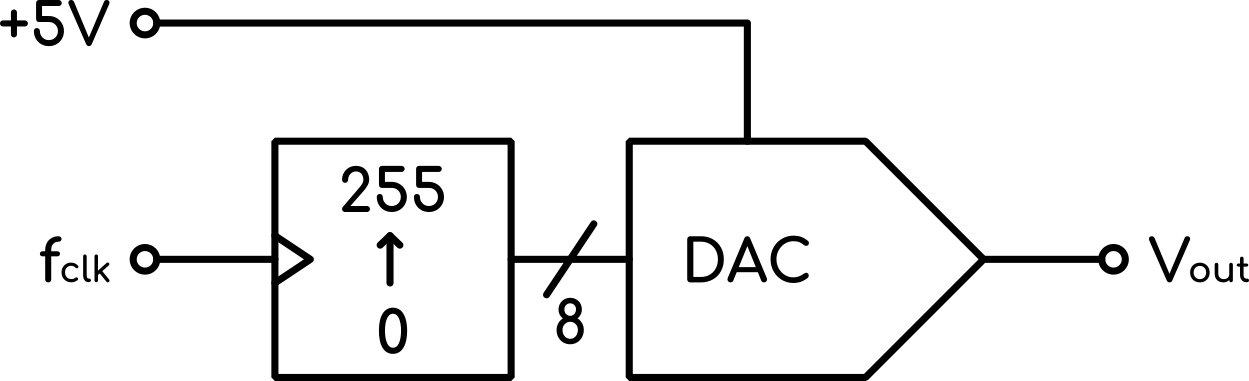
\includegraphics{block_diagrams/ramp_block_diagram.png}
    \caption{Schema a blocchi del sottosistema per la generazione della rampa}
    \label{ramp_block_diagram}
\end{figure}

A questo punto possiamo calcolare le speccifiche del segnale di clock da generare,
andando a vedere quali sono le frequenze desiderate per i segnali audio:

\begin{itemize}
    \item Valore minimo (nota A0): $f_{signal-min}=27.5\ Hz\rightarrow f_{clk-min}\approx7\ kHz$
          a cui corrisponderà un ingresso di $0\ V$;
    \item Valore massimo (nota A8): $f_{signal-max}\approx7\ kHz\rightarrow f_{clk-max}\approx1.8\ MHz$
          a cui corrisponderà un ingresso di $8\ V$;
\end{itemize}

quindi un range di funzionamento esteso lungo 8 ottave.

%--------------------------------------------------------------------------------------------

\subsection*{Componenti Utilizzati e Schemi Elettrici}

%--------------------------------------------------------------------------------------------

Si passa ora alla scelta dei componenti per la realizzazione del blocco circuitale.

\begin{itemize}
    \item Contatore: 74HC590 \cite{74hc590};
    \item DAC: DAC0800 \cite{dac0800};
\end{itemize}

Per il circuito DAC si utilizza lo schema a pg.10 del relativo datasheet del componente.
Tale configurazione ci permette di convertire il dato binario in un valore compreso
nell'intervallo $\pm V_{ref}$, tuttavia si utilizzano un amplificatore operazionale e dei
resistori di valore differente (rispettivamente TL074 \cite{tl074} e $R_L=\bar{R_L}=3.3\ k\Omega$).
Si noti che anche $V_{ref}$ viene scelta diversa rispetto allo schema nel datasheet
(ovvero $+5\ V$), in modo da garantire le specifiche di progetto sul segnale in uscita.

\begin{figure}[H]
    \centering
    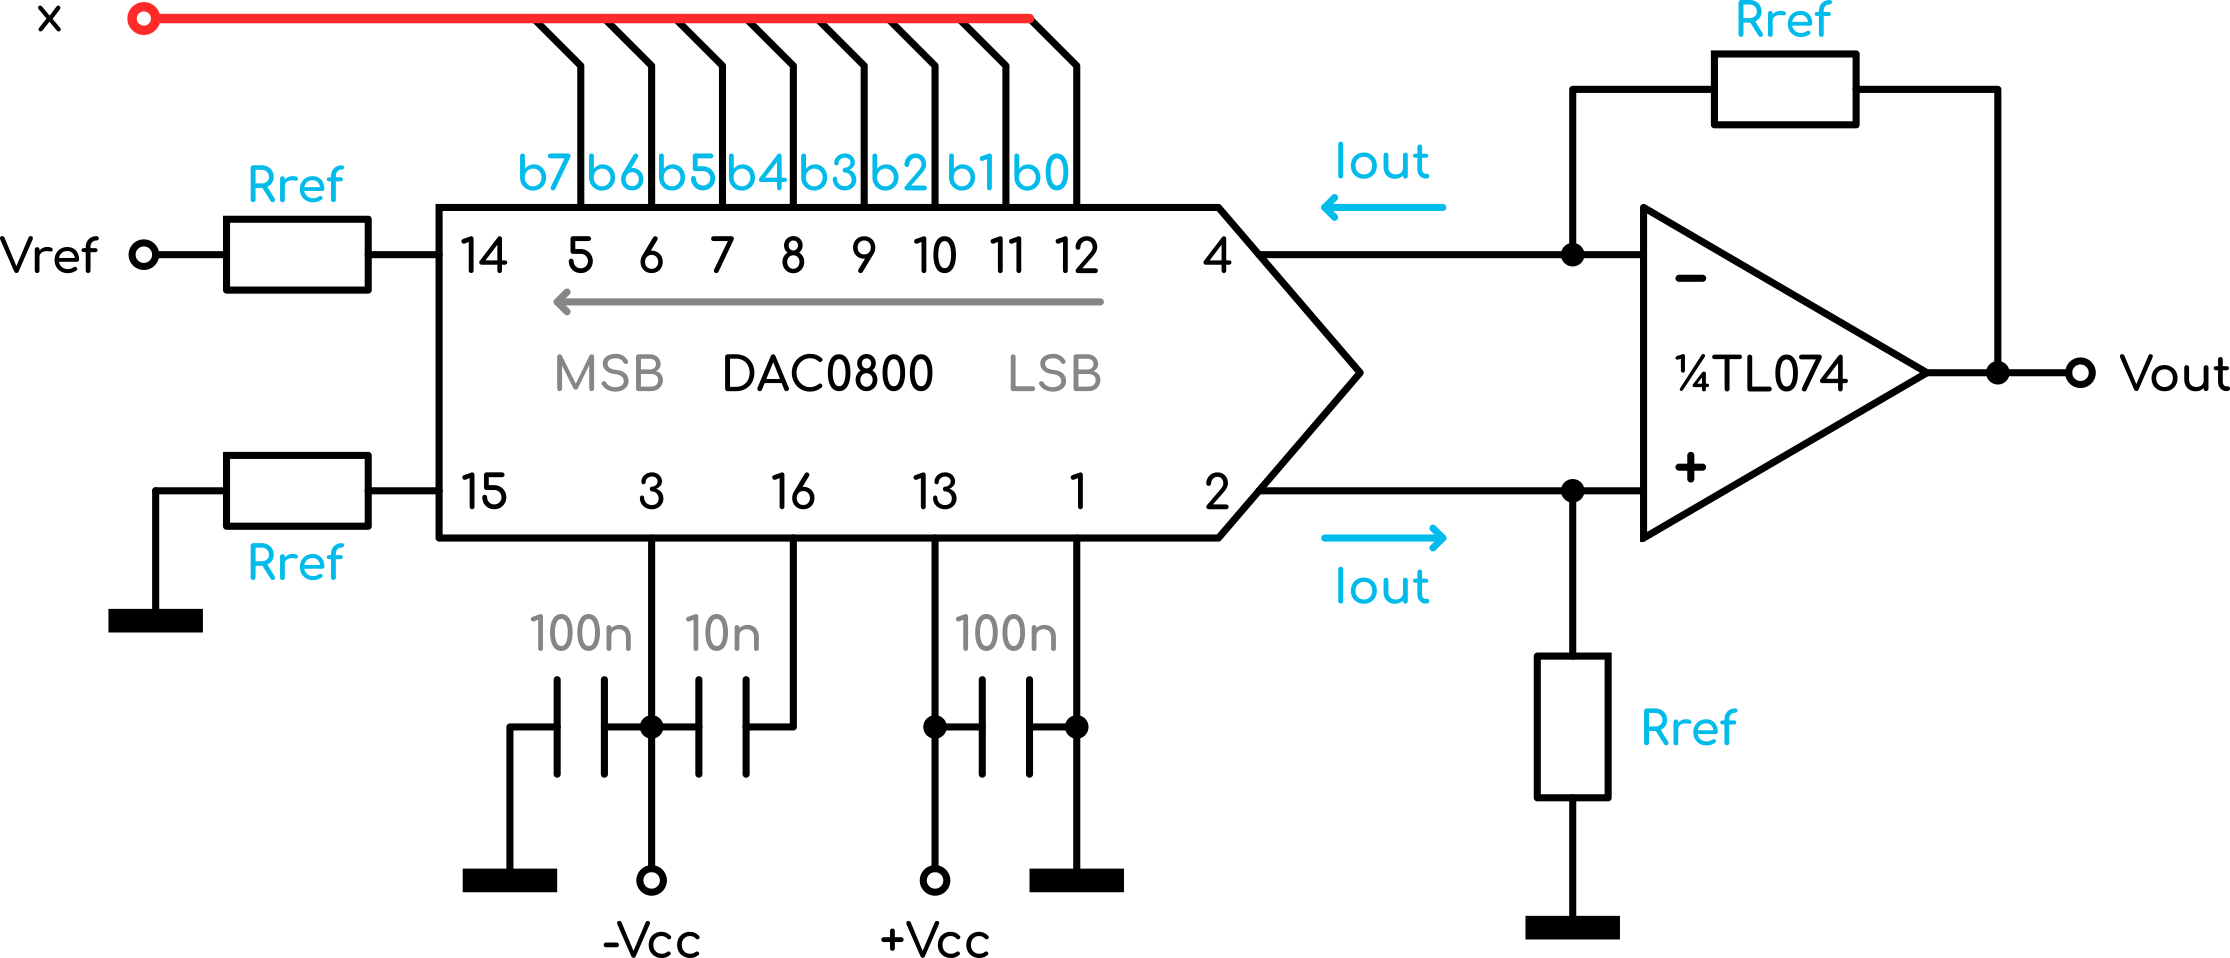
\includegraphics{circuits/DAC_circuit.png}
    \caption{Schema elettrico del DAC, $\pm V_{cc}=\pm 12\ V$}
    \label{DAC_circuit}
\end{figure}

Il DAC eroga una corrente $I_{out}$ proporzionale all'ingresso digitale $x$, che viene poi
convertita in una tensione con un operazionale. Le due grandezze sono legate dalla relazione:

\begin{displaymath}
    V_{out}=V_{ref}\left(\frac{2x-255}{256}\right)=5\left(\frac{2x-255}{256}\right)\ [V]
\end{displaymath}

Il contatore invece viene collegato nel seguente modo:

\begin{figure}[H]
    \centering
    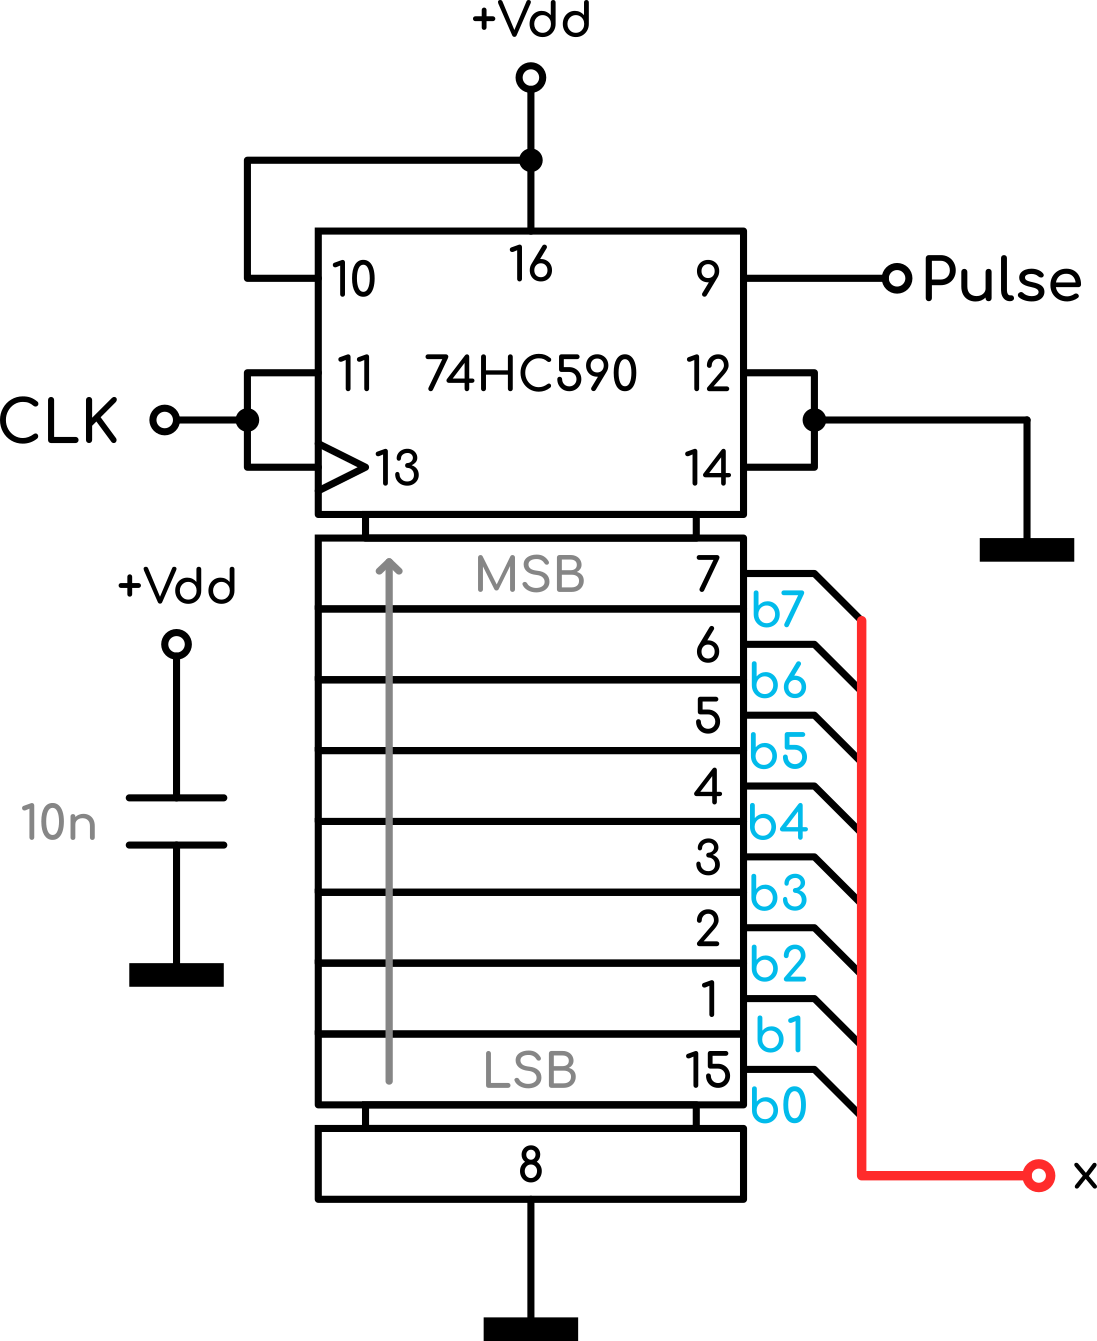
\includegraphics{circuits/ramp_counter_circuit.png}
    \caption{Schema elettrico del contatore per l'onda a rampa, $V_{dd}=+5\ V$}
    \label{ramp_counter_circuit}
\end{figure}

Si noti l'uscita "Pulse" in figura \ref{ramp_counter_circuit} dalla quale viene prelevato
il segnale a impulso precedentemente accennato, discusso più in dettaglio nel capitolo.
%\ref{ch_impulso}.

Infine, collegando i due blocchi insieme, l'andamento di $V_{out}$ sarà simile a quello
rappresentato in figura \ref{high_res_ramp}, e ad ogni impulso di clock corrisponderà un
gradino di tensione di circa $40\ mV$ come calcolato precendentemente.

%--------------------------------------------------------------------------------------------

\subsection*{Risultati Pratici}

%--------------------------------------------------------------------------------------------

Andiamo ora a verificare la correttezza del circuito realizzato con il seguente setup di
misura:

\begin{figure}[H]
    \centering
    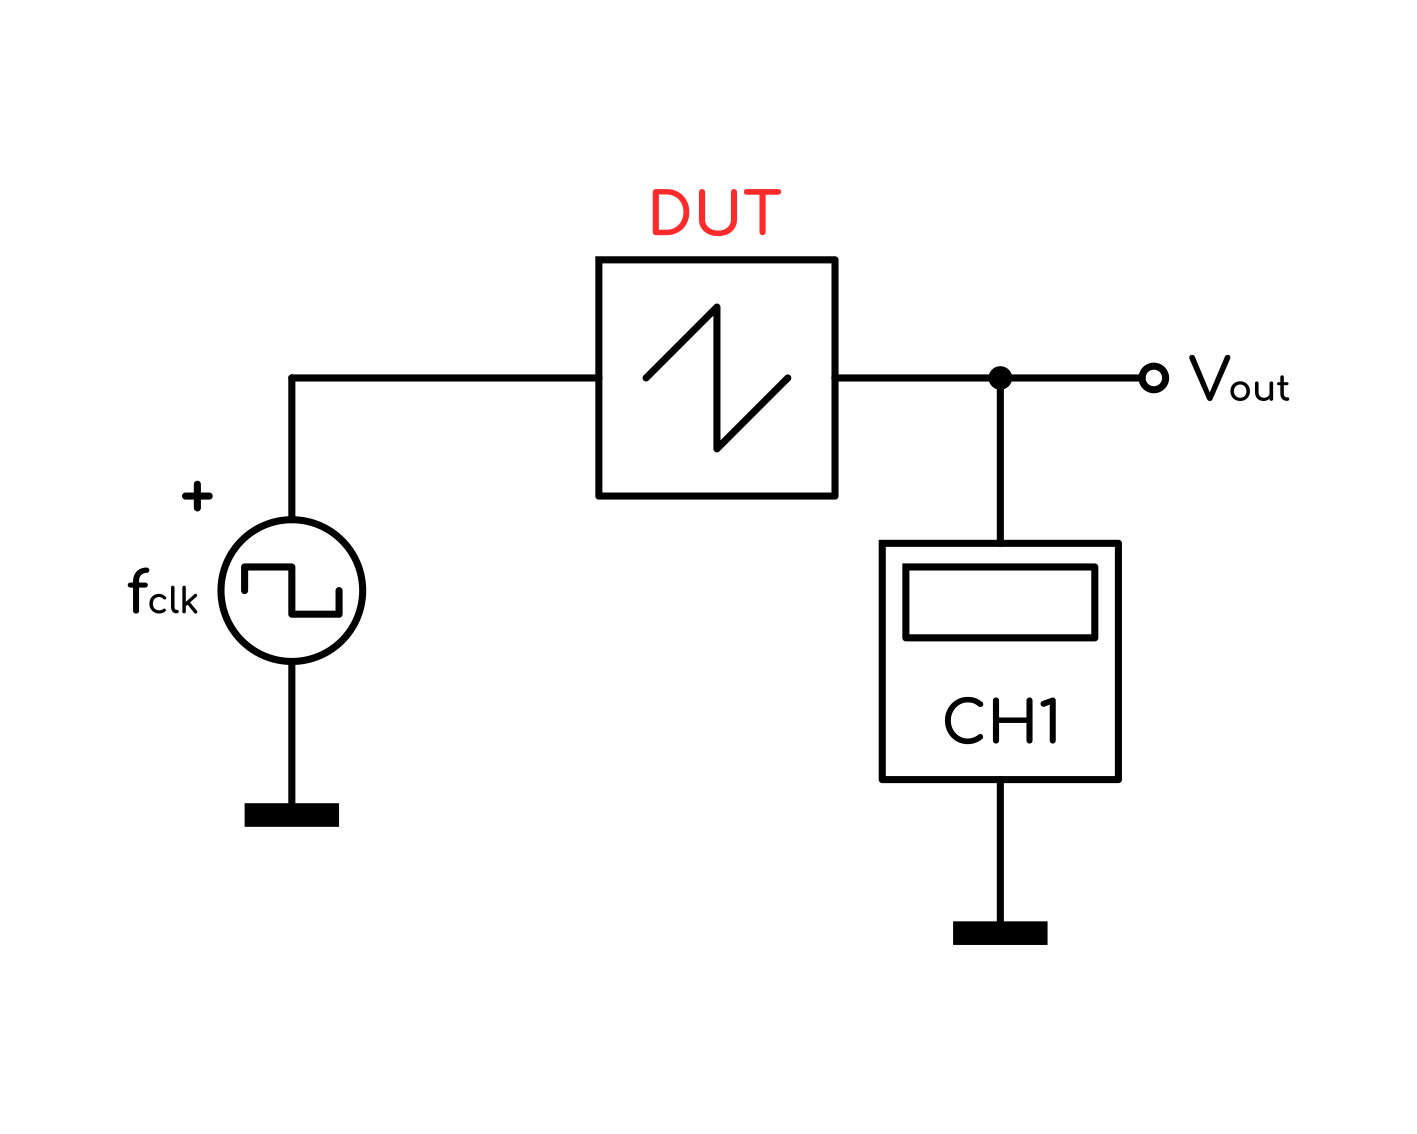
\includegraphics{block_diagrams/mis_ramp.png}
    \caption{Circuito di misura del segnale rampa}
    \label{mis_ramp}
\end{figure}

\vspace{2cm}

Si osservano le seguenti forme d'onda:

\begin{figure}[H]
    \centering

    \begin{subfigure}{.5\textwidth}
        \centering
        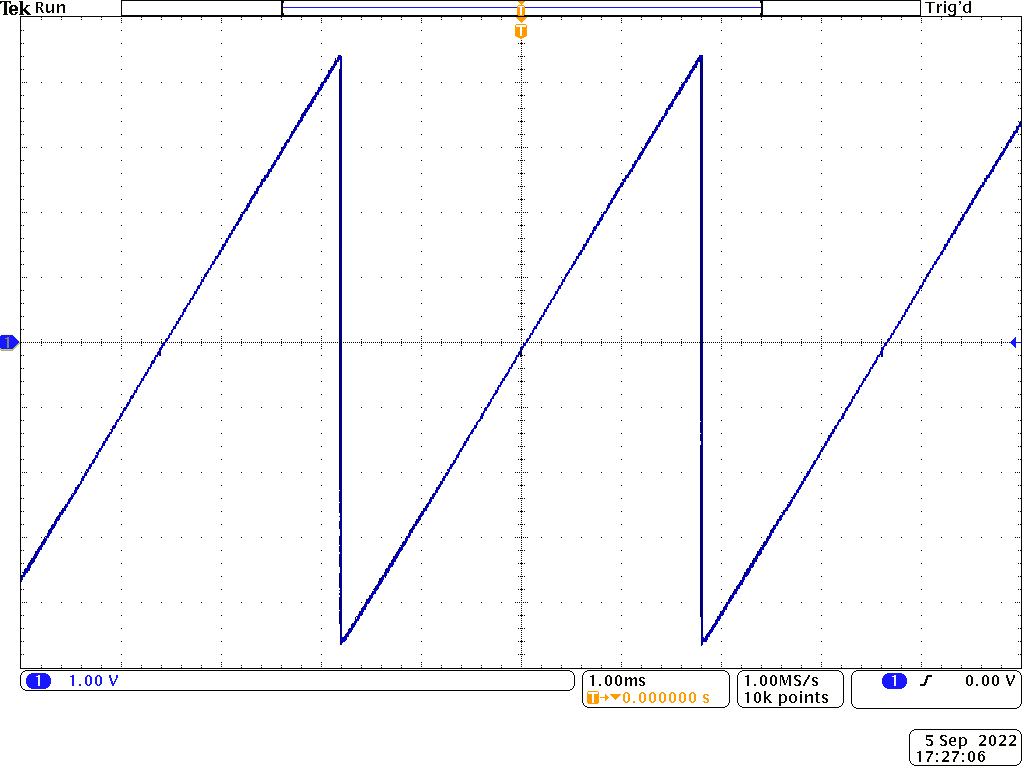
\includegraphics[scale = 0.2]{acquisitions/ramp_wave.png}
        \caption{Acquisizione del segnale a rampa ottenuto}
        \label{acq_ramp}
    \end{subfigure}%
    \begin{subfigure}{.5\textwidth}
        \centering
        
\includegraphics{misc/oscilloscope_placeholder.png}
        \caption{Zoom degli step della rampa e clock}
        \label{acq_ramp_steps}
    \end{subfigure}

    \caption{Correttezza del circuito per il segnale a rampa}
    \label{acq_ramp_signals}
\end{figure}

%--------------------------------------------------------------------------------------------

\section{Triangolo}

%--------------------------------------------------------------------------------------------

\subsection*{Principio di Funzionamento}

%--------------------------------------------------------------------------------------------

Il ragionamento è del tutto analogo a quello del contatore per la rampa, tuttavia in questo
caso il contatore utilizzato è bidirezionale (quindi in grado di contare da $0$ a $2^n$ e
viceversa) e necessita di un segnale che determini la direzione di conteggio (Up o Down).

\begin{figure}[H]
    \centering
    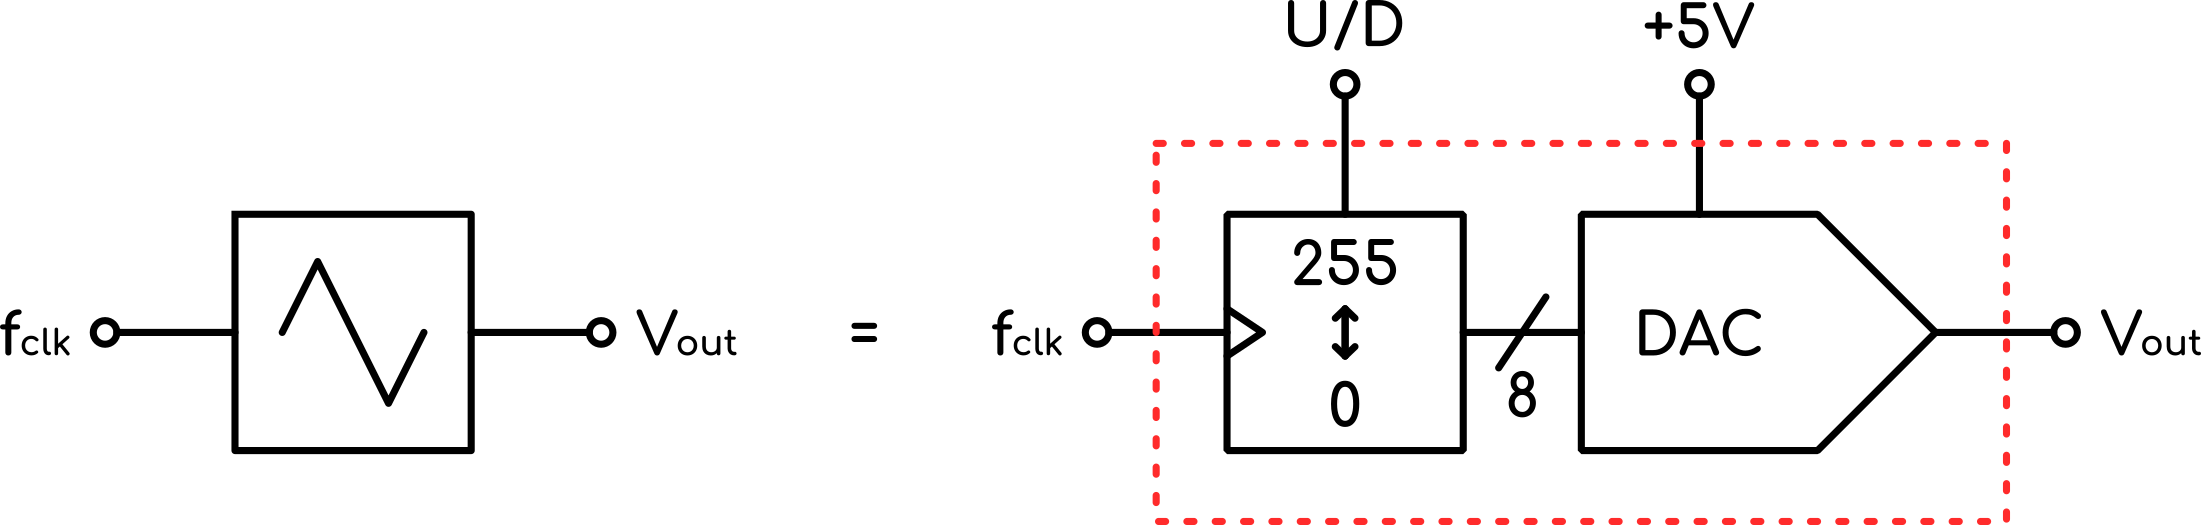
\includegraphics{block_diagrams/triangle_block_diagram.png}
    \caption{Schema a blocchi del sottosistema per la generazione del triangolo}
    \label{triangle_block_diagram}
\end{figure}

\begin{figure}[H]
    \centering

    \begin{subfigure}{.5\textwidth}
        \centering
        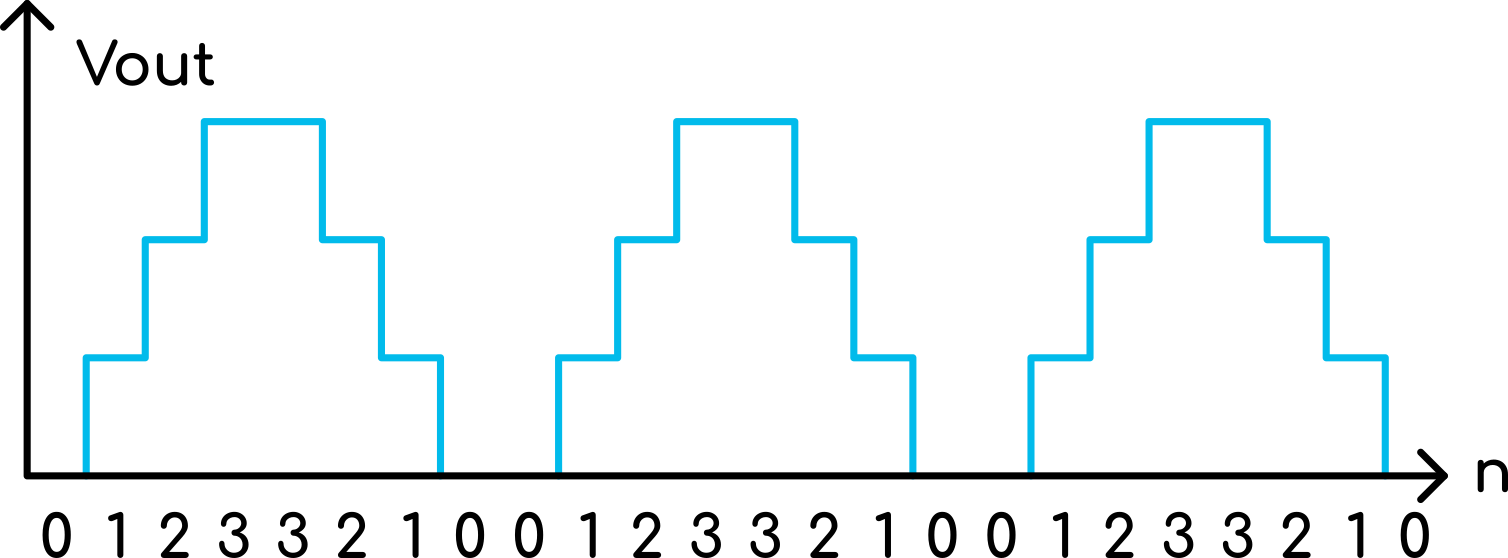
\includegraphics{graphs/low_res_triangle.png}
        \caption{Triangolo ottenuto con un contatore a 2 bit}
        \label{low_res_triangle}
    \end{subfigure}%
    \begin{subfigure}{.5\textwidth}
        \centering
        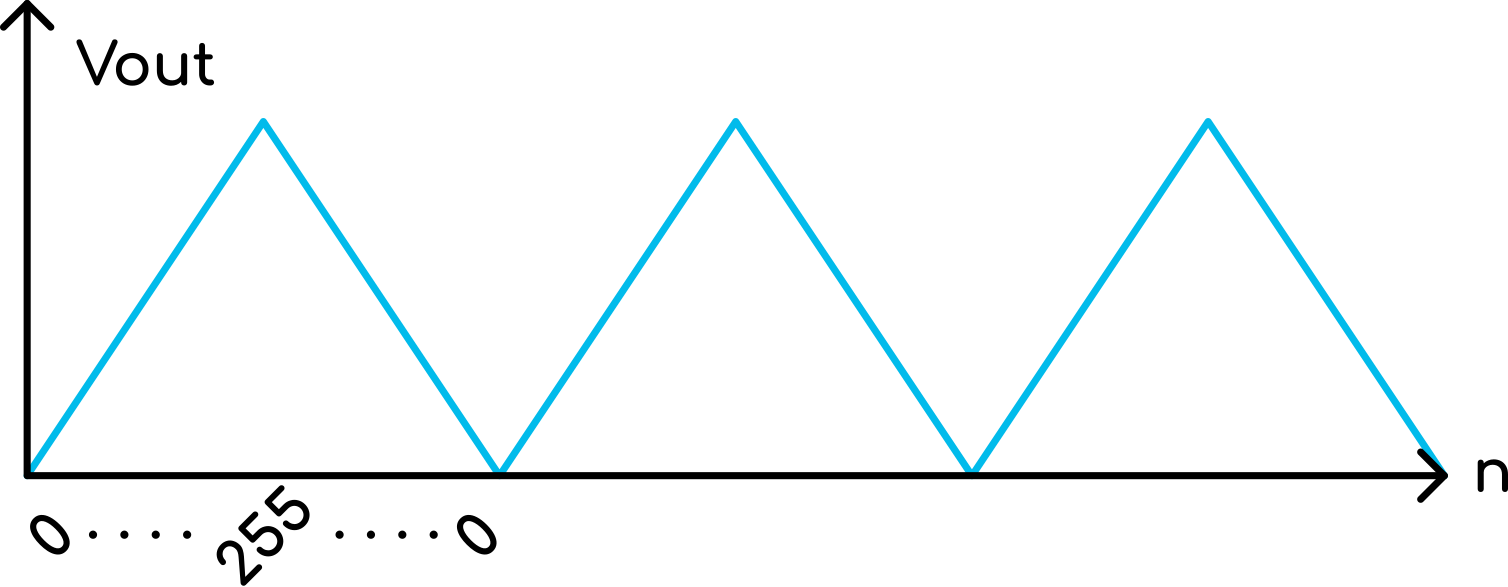
\includegraphics{graphs/high_res_triangle.png}
        \caption{Triangolo ottenuto con un contatore a 8 bit}
        \label{high_res_triangle}
    \end{subfigure}

    \caption{Confronto tra contatori bidirezionali con diverso numero di bit}
    \label{triangles}
\end{figure}

La configurazione del DAC rimane quella utilizzata per la rampa e rappresentata in figura
\ref{DAC_circuit}. In questo caso tuttavia il numero di cicli di clock utilizzati è doppio
rispetto a quello per la rampa, poichè dovranno essere eseguiti 256 conteggi verso l'alto
e 256 conteggi verso il basso per ottenere un singolo periodo di onda triangolare. Ne
consegue quindi che anche la frequenza di clock in ingresso a questo sottosistema dovrà
essere doppia rispetto alla rampa, come risulta evidente in figura \ref{steps}.

\begin{figure}[H]
    \centering

    \begin{subfigure}{.5\textwidth}
        \centering
        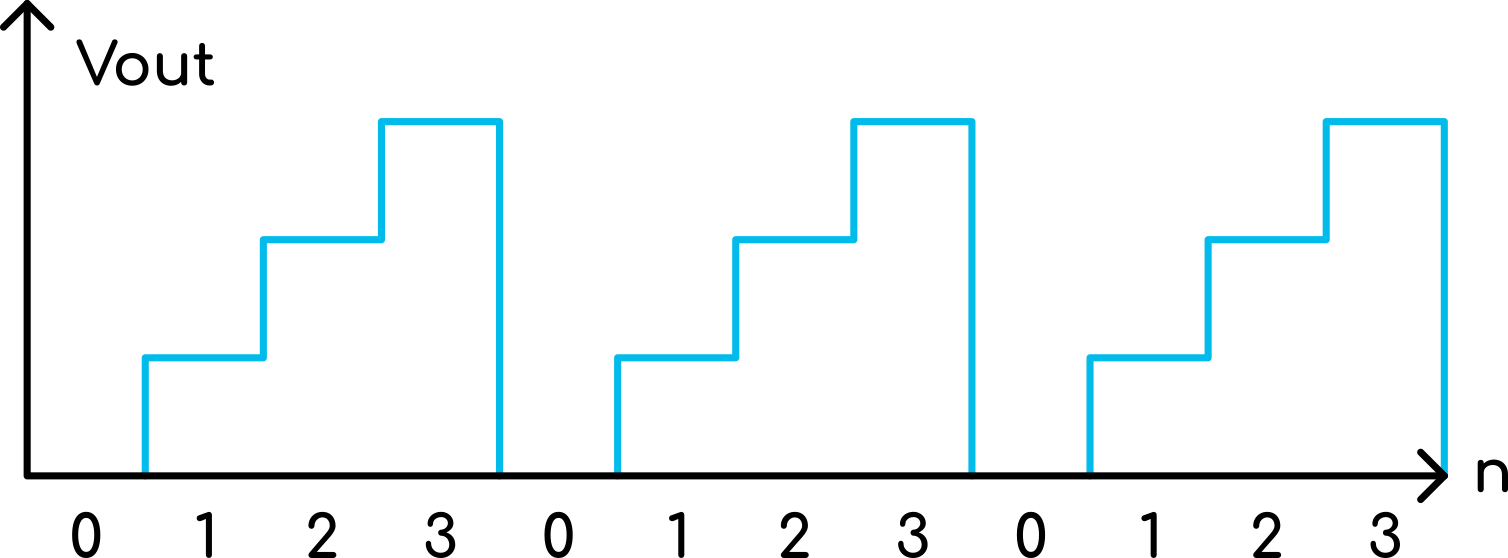
\includegraphics{graphs/low_res_ramp.png}
        \caption{Rampa ottenuta con un contatore a 2 bit}
    \end{subfigure}%
    \begin{subfigure}{.5\textwidth}
        \centering
        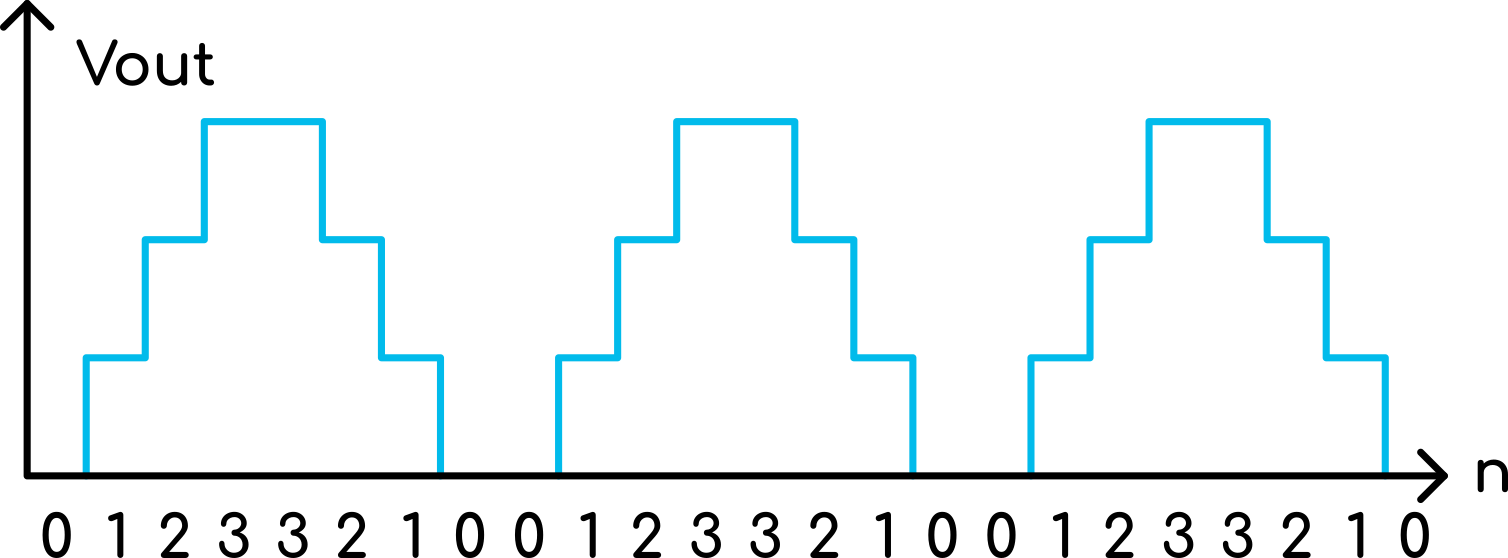
\includegraphics{graphs/low_res_triangle.png}
        \caption{Triangolo ottenuto con un contatore a 2 bit}
    \end{subfigure}

    \caption{Confronto del conteggio tra contatori unidirezionali (a) e bidirezionali (b)}
    \label{steps}
\end{figure}

%--------------------------------------------------------------------------------------------

\subsection*{Componenti Utilizzati e Schemi Elettrici}

%--------------------------------------------------------------------------------------------

L'unico componente diverso rispetto al circuito per la rampa è il contatore, che come già
detto deve essere bidirezionale. Si utilizzano due 74LS169 \cite{74ls169} in cascata nella
seguente configurazione:

\begin{figure}[H]
    \centering
    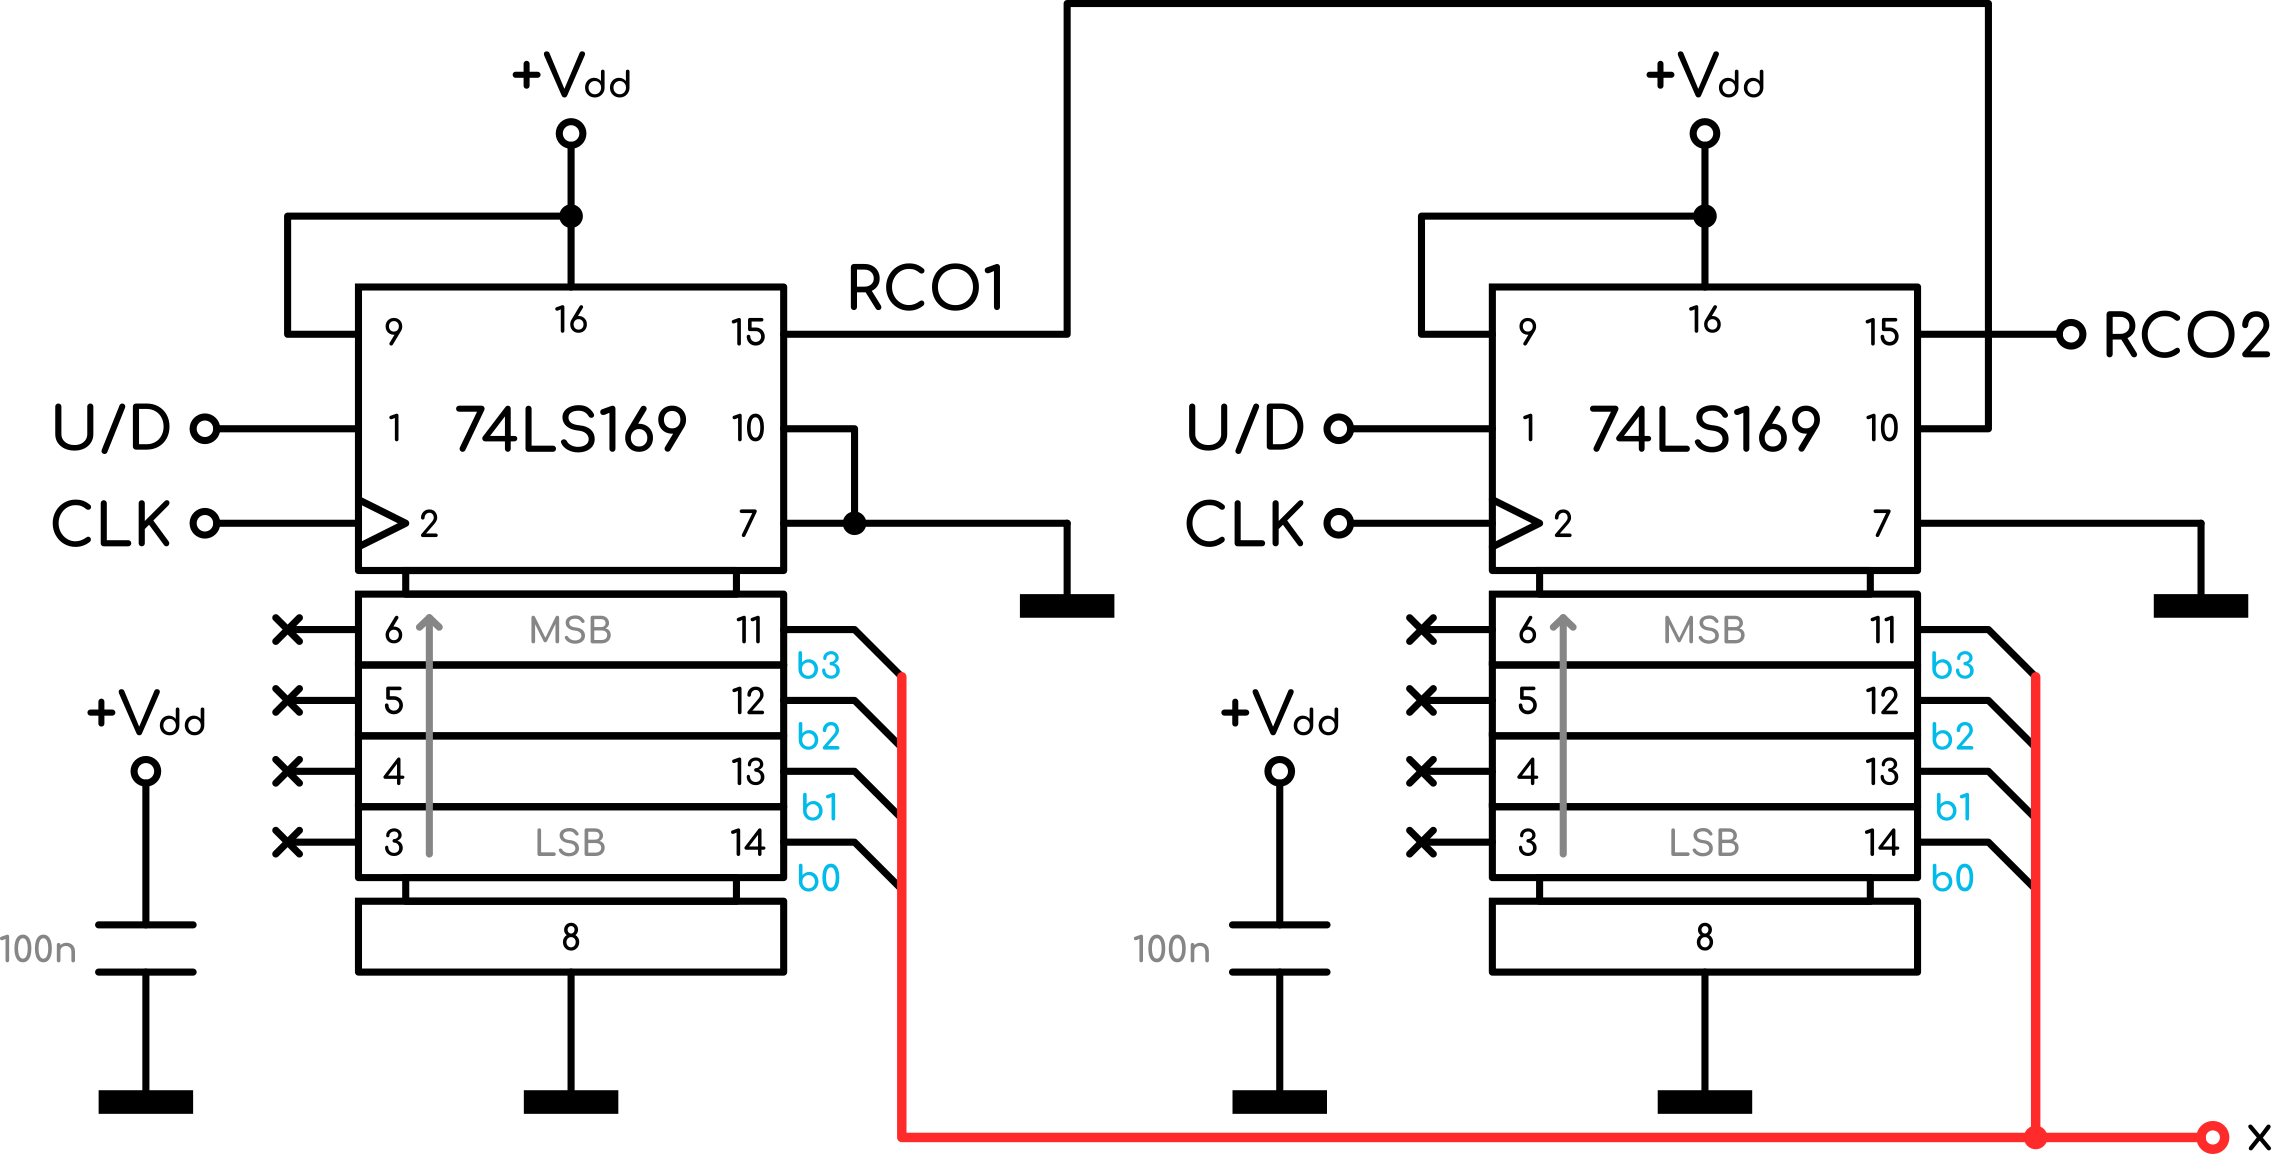
\includegraphics{circuits/triangle_counter_circuit.png}
    \caption{Schema elettrico dei contatori per l'onda triangolare, $V_{dd}=+5\ V$}
    \label{triangle_counter_circuit}
\end{figure}

Il componente utilizzato presenta anche degli ingressi per il preset del numero di partenza
(pin da 3 a 6), che però nel nostro caso non vengono utilizzati.

L'uscita denominata $RCO2$ verrà utilizzata per pilotare il verso del conteggio, essa infatti
commuta durante il ciclo di clock corrispondente al conteggio precedente all'overflow, ovvero
$255$ in modalità "Up" e $0$ in modalità "Down".

%--------------------------------------------------------------------------------------------

\subsection*{Risultati Pratici}

%--------------------------------------------------------------------------------------------

Si verifica ora la correttezza del circuito realizzato utilizzando il setup di misura seguente:

\begin{figure}[H]
    \centering
    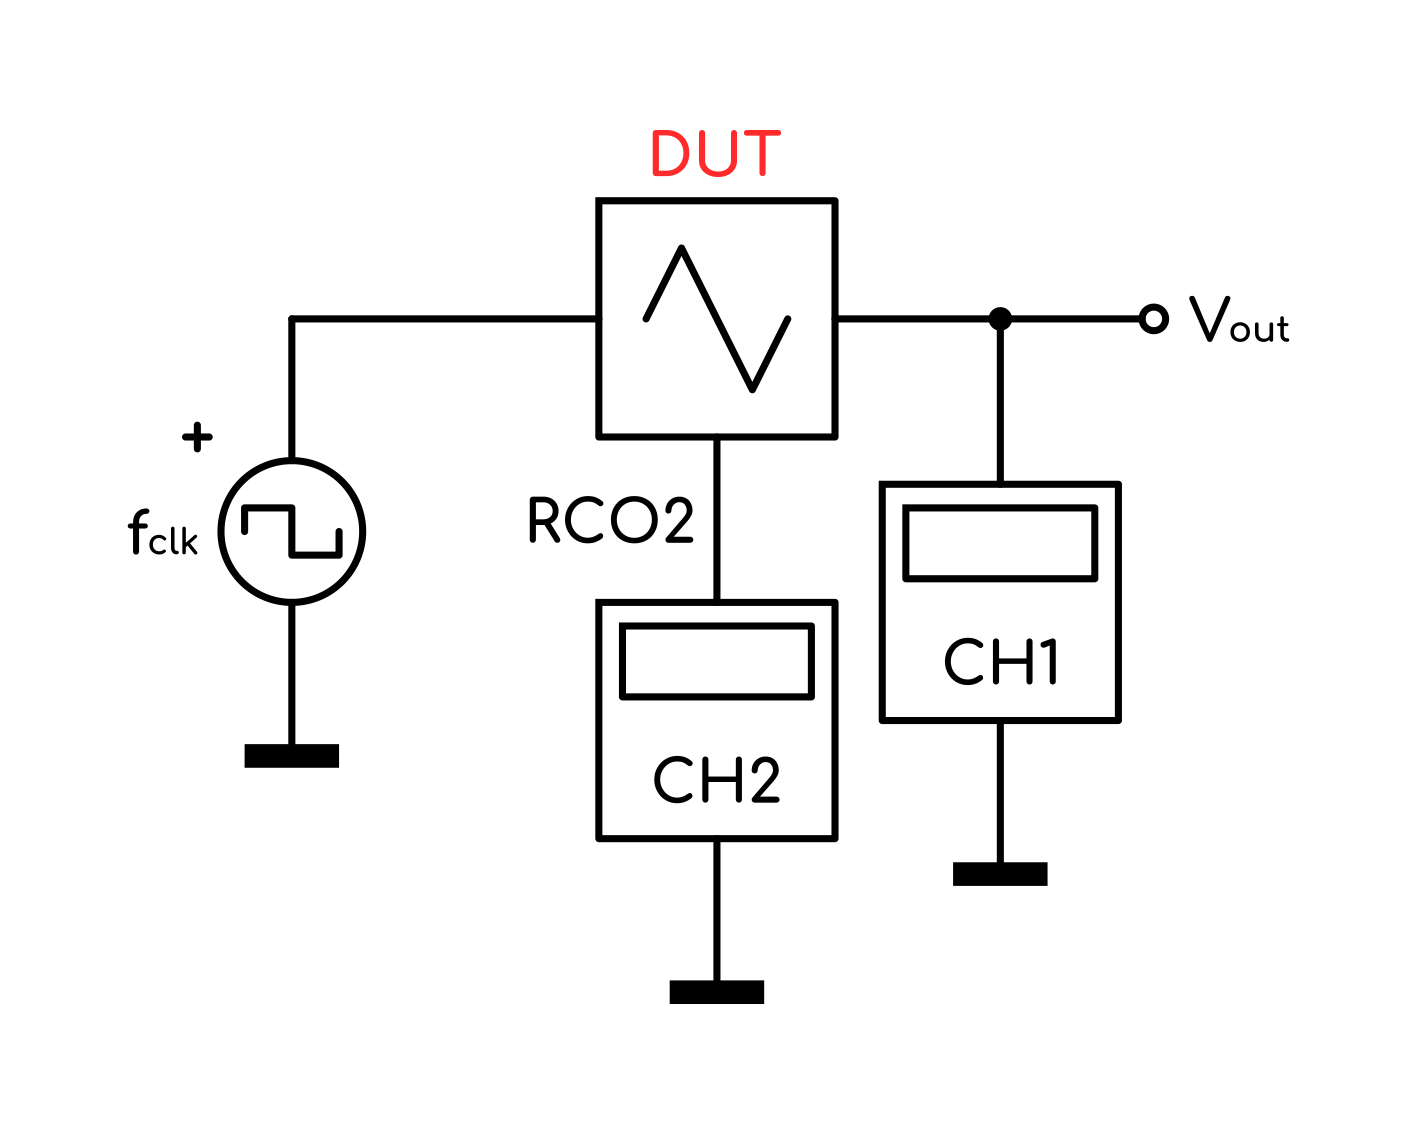
\includegraphics{block_diagrams/mis_triangle.png}
    \caption{Circuito di misura del segnale triangolo}
    \label{mis_triangle}
\end{figure}

Si osservano le seguenti forme d'onda:

\begin{figure}[H]
    \centering

    \begin{subfigure}{.5\textwidth}
        \centering
        
\includegraphics{misc/oscilloscope_placeholder.png}
        \caption{Acquisizione del segnale a triangolo ottenuto}
        \label{acq_triangle}
    \end{subfigure}%
    \begin{subfigure}{.5\textwidth}
        \centering
        
\includegraphics{misc/oscilloscope_placeholder.png}
        \caption{Zoom degli step del triangolo acquisito e clock}
        \label{acq_triangle_steps}
    \end{subfigure}

    \caption{Correttezza del circuito per il segnale a triangolo}
    \label{acq_triangle_signals}
\end{figure}

%--------------------------------------------------------------------------------------------

\section{Adattamento dei Segnali di Clock e Pilotaggio}

%--------------------------------------------------------------------------------------------

Si è visto come, per avere la stessa frequenza di segnale d'uscita, il contatore del
triangolo deve avere una frequenza di clock doppia rispetto a quella del contatore della
rampa. Questo problema si risolve facilmente inserendo prima del contatore unidirezionale
un divisore di frequenza, ottenuto con un semplice toggle flip-flop (TFF).

\begin{figure}[H]
    \centering
    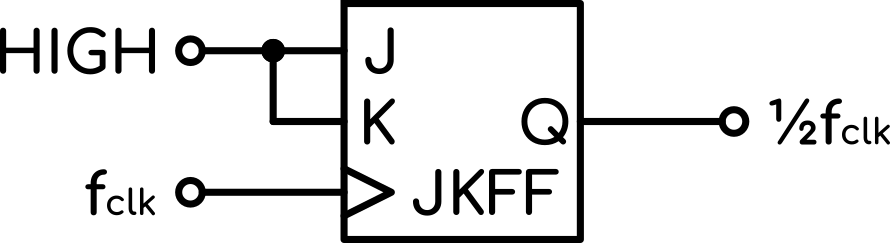
\includegraphics{block_diagrams/freq_divider_block_diagram.png}
    \caption{Schema a blocchi del divisore di frequenza}
    \label{freq_divider_block_diagram}
\end{figure}

Le specifiche sul segnale di clock ci impongono allora di generare un segnale a onda quadra
con frequenza variabile nel range $(14\ kHz,3.6\ MHz)$, in modo che ½$f_{clk}$ abbia
i valori di frequenza precedentemente calcolati.

Invece, per fare in modo che il contatore del triangolo cambi effettivamente verso di conteggio
è necessario utilizzare un altro TFF utilizzando come ingresso $\overline{RCO2}$ (poichè
attivo a livello logico basso) e connesso all'ingresso $U/D$ del contatore.

\begin{figure}[H]
    \centering
    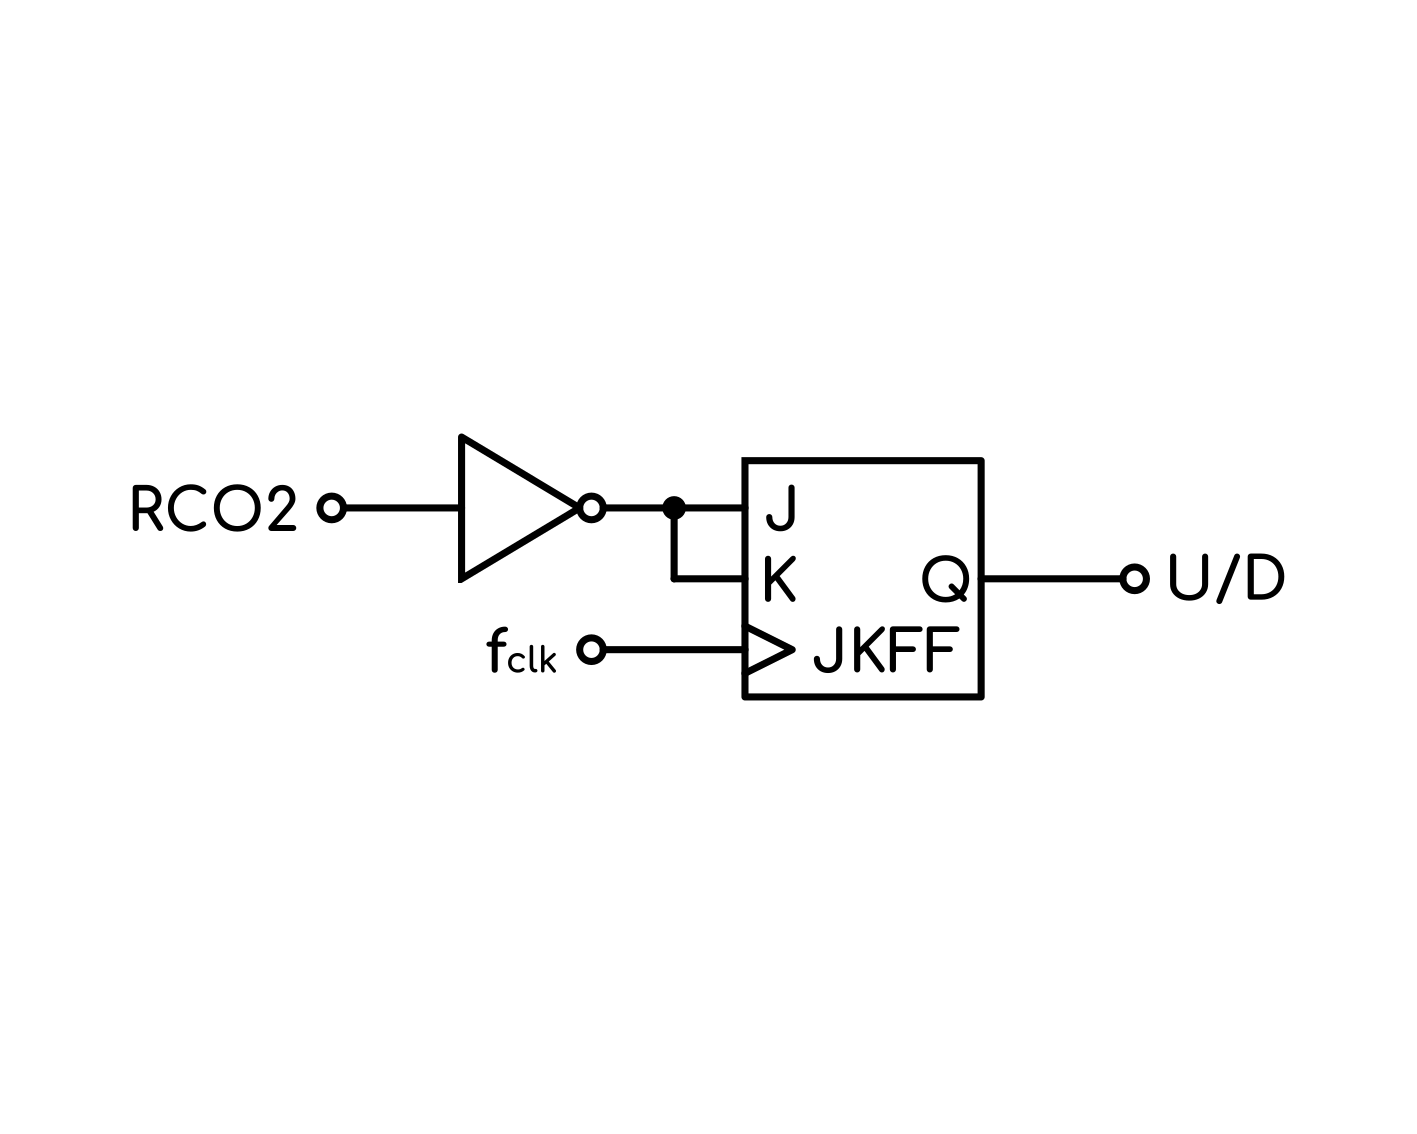
\includegraphics{block_diagrams/UD_block_diagram.png}
    \caption{Schema a blocchi del sistema per il segnale di pilotaggio}
    \label{UD_block_diagram}
\end{figure}

I componenti utilizzati per questo scopo sono:

\begin{itemize}
    \item Flip-Flop: 74HC73 \cite{74hc73};
    \item MOSFET: 2N7000 \cite{2n7000};
\end{itemize}

Lo schema elettrico per l'inverter è rappresentato in figura \ref{inverter_circuit}, dove
il MOSFET utilizzato è compatibile con le tensioni logiche presenti nel circuito.

\begin{figure}[H]
    \centering
    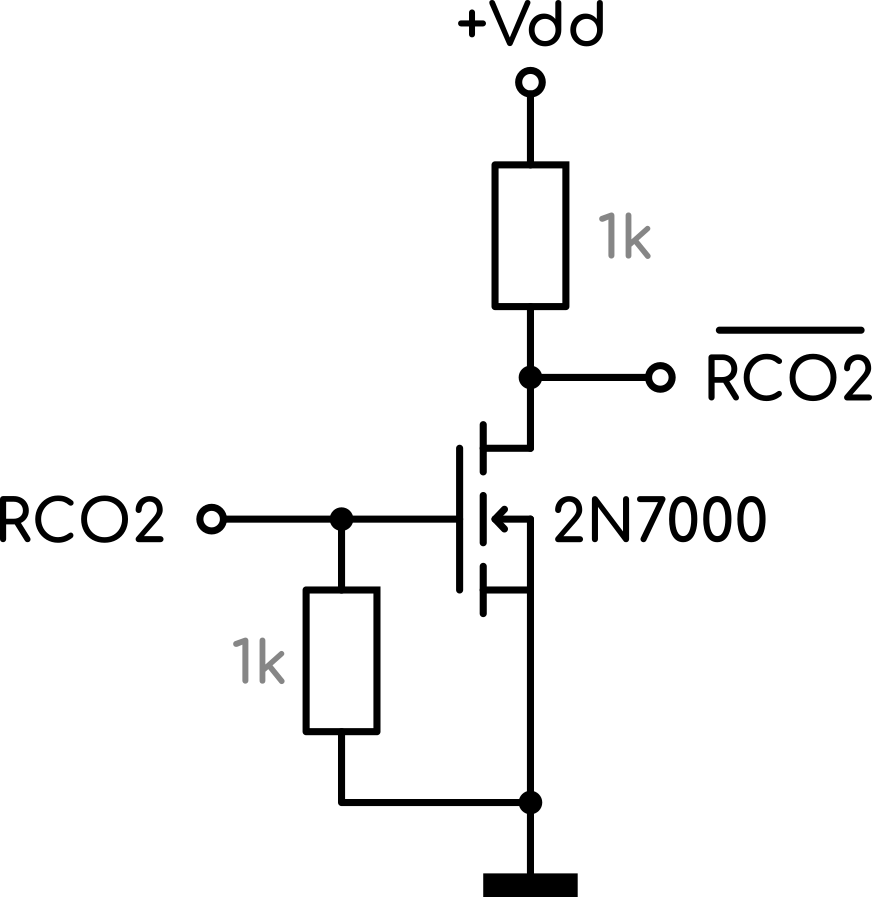
\includegraphics{circuits/inverter_circuit.png}
    \caption{Schema elettrico dell'inverter logico, $V_{dd}=+5\ V$}
    \label{inverter_circuit}
\end{figure}

%--------------------------------------------------------------------------------------------

\subsection*{Risultati Pratici}

%--------------------------------------------------------------------------------------------

Si verifica la correttezza dei circuiti:

\begin{figure}[H]
    \centering

    \begin{subfigure}{.5\textwidth}
        \centering
        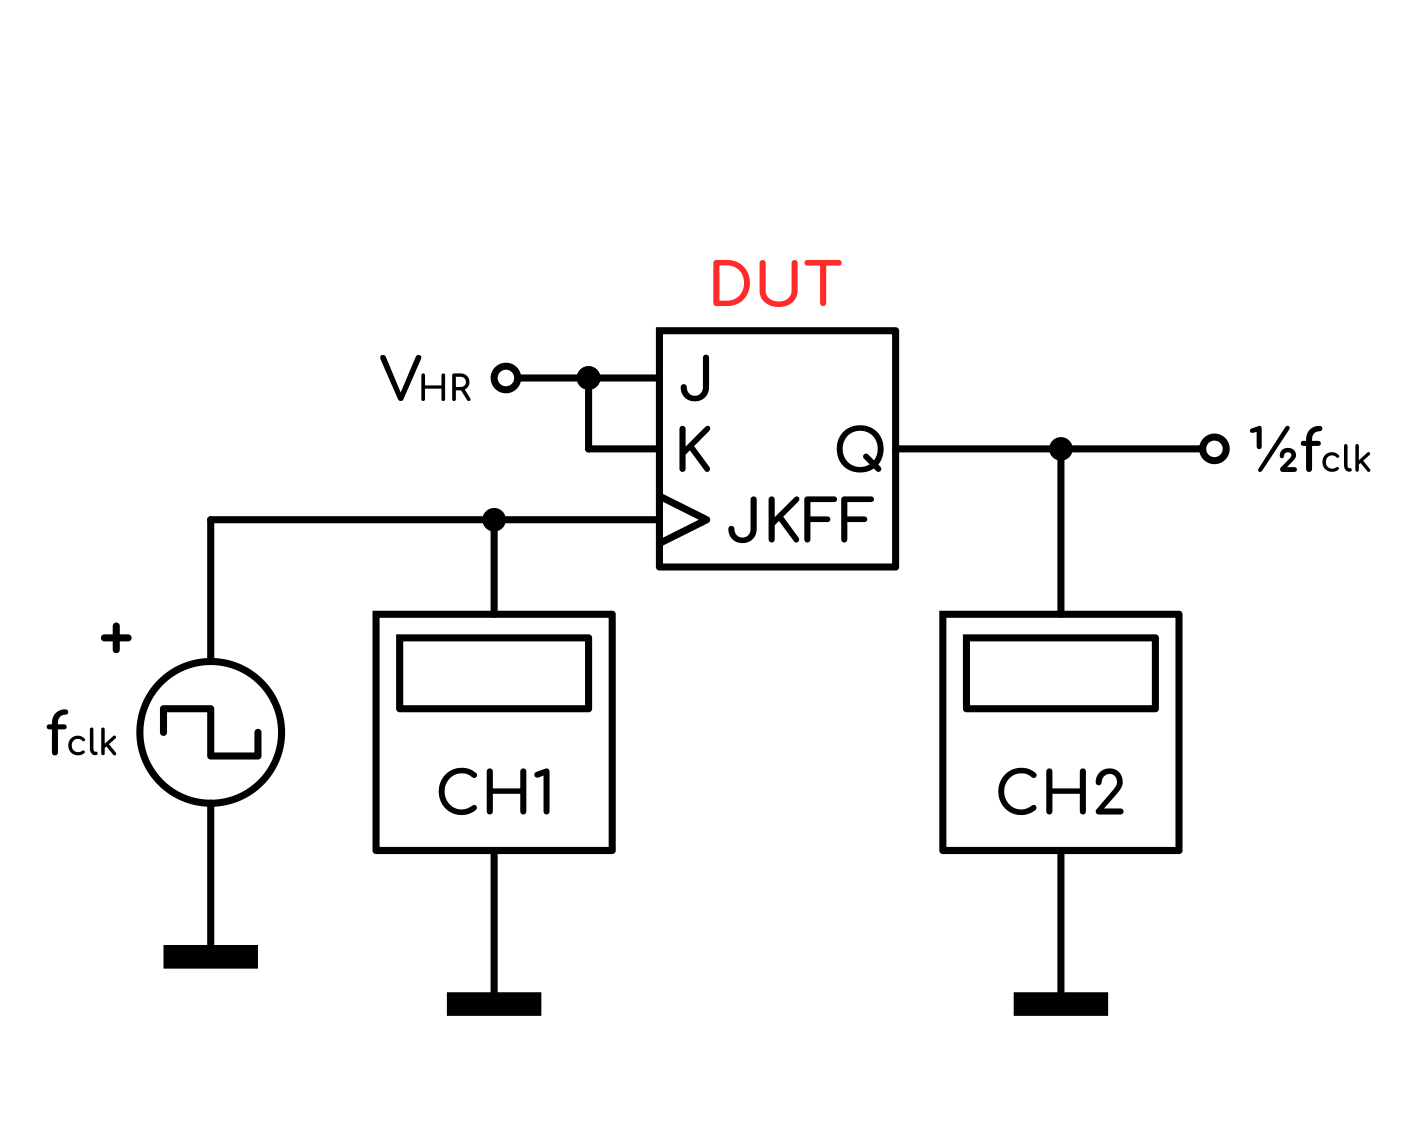
\includegraphics{block_diagrams/mis_clock_divider.png}
        \caption{Circuito di misura del divisore di frequenza}
        \label{mis_clock_divider}
    \end{subfigure}%
    \begin{subfigure}{.5\textwidth}
        \centering
        
\includegraphics{misc/oscilloscope_placeholder.png}
        \caption{Acquisizione dei segnali $f_{clk}$ e ½$f_{clk}$}
        \label{acq_clock_divider}
    \end{subfigure}

    \caption{Correttezza del circuito divisore di frequenza}
    \label{clock_divider}
\end{figure}

\begin{figure}[H]
    \centering

    \begin{subfigure}{.5\textwidth}
        \centering
        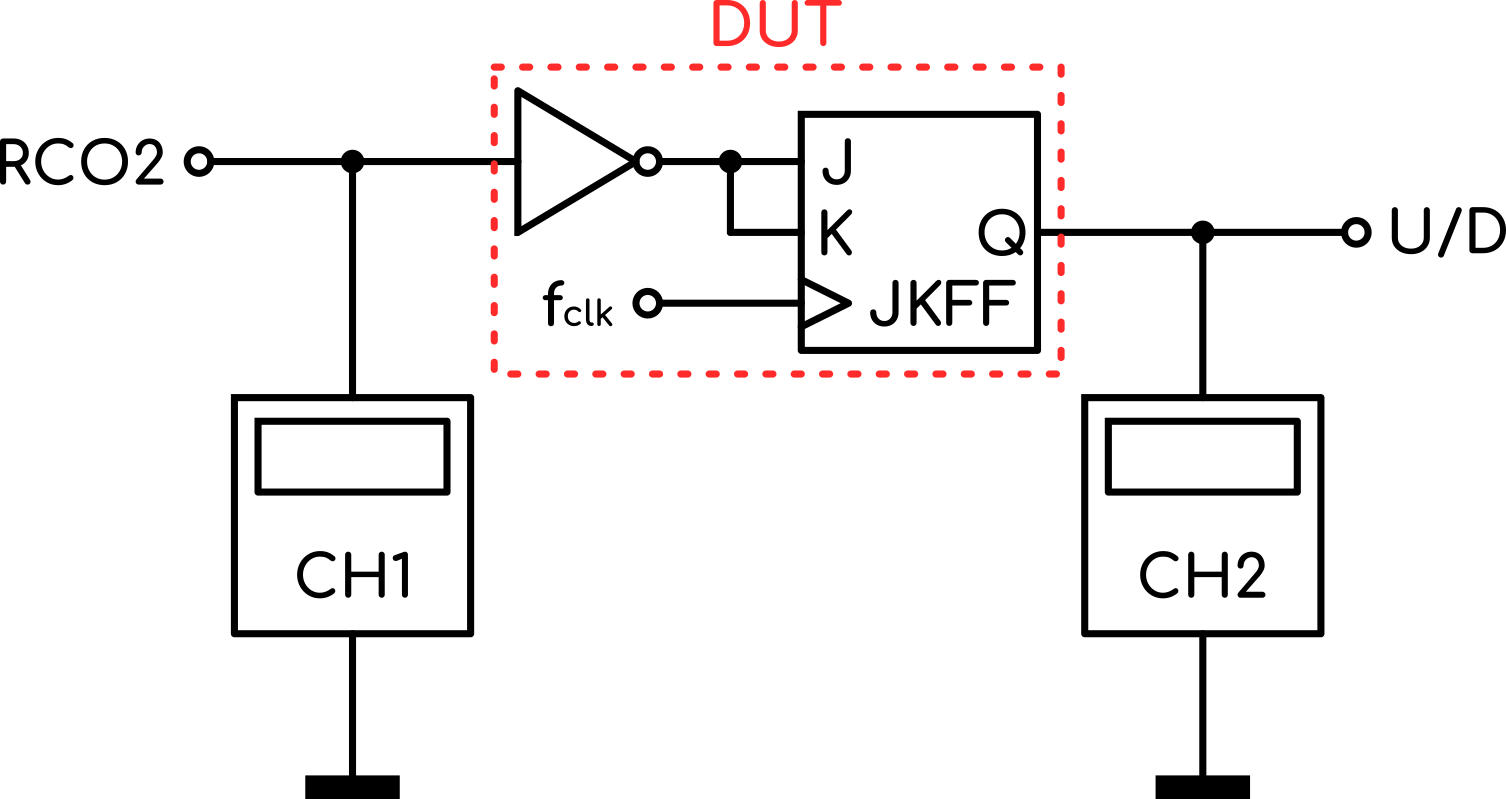
\includegraphics{block_diagrams/mis_UD.png}
        \caption{Circuito di misura del segnale $U/D$}
        \label{mis_UD}
    \end{subfigure}%
    \begin{subfigure}{.5\textwidth}
        \centering
        
\includegraphics{misc/oscilloscope_placeholder.png}
        \caption{Acquisizione dei segnali $RCO2$ e $U/D$}
        \label{acq_UD}
    \end{subfigure}

    \caption{Correttezza del circuito di pilotaggio del contatore up-down}
    \label{UD}
\end{figure}

%--------------------------------------------------------------------------------------------
